\begin{figure}[!h]
    \centering
    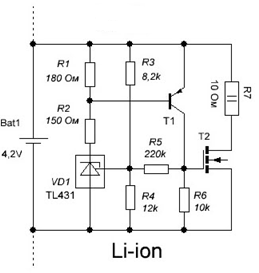
\includegraphics[width=0.4\linewidth]{img/chem_pass_tl431.png}
    \caption{Схема пассивной балансировки на чипе TL-431}
    \label{fig:tl431}
\end{figure}

Данный метод прост в реализации. На каждую ячейку приходится балансировочный резистор 
и небольшая автоматическая обвязка, которая включает балансировку в нужном диапазоне напряжений.
Для примера можно расмотреть схему на базе чипа TL-431. (Рис.\ref{fig:tl431}). (Подробнее в статье \cite{8898267})

